\chapter{Empirical Studies}
\label{ch:empirical-studies}

\section{Introduction}
In this section we include the analysis of two of the techniques used in the project: the Viola-Jones method and the Convolutional Neural Networks. In order to prove their effectiveness we will perform an experiment for each of them. The experiments have been fully documented, including the data set used and the results, which are discussed at the end.

\section{Experiment 1: Effectiveness of Viola-Jones method for Face Detection}
	\subsection{Objective}
	As it was already explained in the Research section (\ref{subsec:face_detec_techniques}), the Viola-Jones method "stands out for performing a high detection rate with a very low false positive rate and it is capable to work in a real time situation". These features have made it widely used in the recent years and it was also the reason why it was finally chosen for this project. 

	In this experiment, we are going to test this affirmation by applying the method to a certain set of images. It will be composed of an equal proportion of face images, near-face images from a human perspective and non-face images. The results will be displayed including the faces that were correctly detected, the faces that were missed (i.e. false negatives) and the images incorrectly classified as having a face, when they did not (i.e. false positives).

	\subsection{Method and parameters}
	The computer used to run the experiment is a laptop Toshiba C50-A-1GU with a 2,40 GHz Intel Processor Core i3-4000M, 8GB 1600MHz RAM memory and Kubuntu 17.10 OS (Linux kernel version 4.13.0-38-generic). The Viola-Jones method  is applied using the OpenCV library as it was done in the \textit{Intelligent Assistant}. In fact, the code used for this experiment (Figure \ref{fig:fd_experiment_code}) is pretty similar to the included in the \textit{face{\_}detection} module, discussed in the Design chapter (\ref{subsec:face_det}).

	\begin{figure}[!ht]
		\centering
		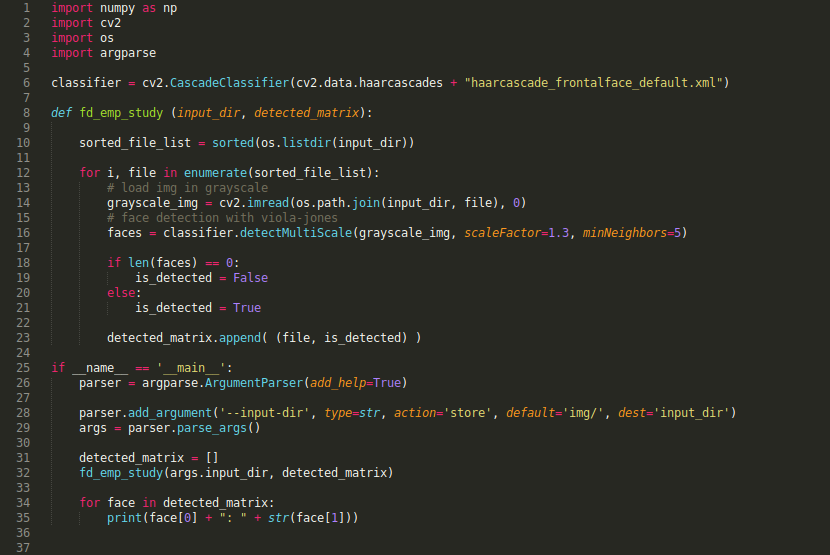
\includegraphics[width=14cm]{emp_studies/fd_experiment_code}
		\caption{Code used to run the Experiment 1}
		\label{fig:fd_experiment_code}
	\end{figure}

	The images are located in a folder named "img", in the same directory as the file. The filename of these images indicates the group to which it belongs and the id of the image, an integer of 2 units filled with zeros if necessary. Then, the filename of the images follow one of these patterns: "face{\_}XX.jpg", "near-face{\_}XX.jpg" or "non-face{\_}XX.jpg".

	The classifier selected for this task is "haarcascade{\_}frontface{\_}default", the same used in the application. The images are loaded in grayscale and the classifier is applied to perform the face detection. This method returns an array with the location of the detected faces in the image, so evaluating its length, we know whether the classifier detected a face or not (i.e. the array would be empty). 

	\subsection{Data set}
	The dataset used in the experiment is composed of a total of 90 images, where 30 of them contain a human face, 30 contain a pattern that humans could interpret as face and 30 do not contain any face. In the Figure \ref we can see the complete dataset. All images are square-shaped with a resolution of 250x250 pixels. The face images belong to the \gls{lfw} dataset (\cite{lfw_db}), while near-face images and non-face images were obtained using Google images and after cropped manually.

	The non-face images were obtained after searching for the keys "background" and "abstract wallpaper". The near-face dataset must be explained in detail because the subjective decission of whether the image look like a face enough or not. This group of photos is internally divided in another three sub-groups:

	\begin{itemize}
		\item Images from 1 to 11. The first contain pencil or graphic drawings that represent persons looking straight forward.
		\item Images from 12 to 20. The second group contain cropped faces from paintings that may have variations in the proportions of some face features. 
		\item Images from 21 to 30. The third and last group contain photos from faces of real sculptures.
	\end{itemize}

	%\begin{figure}[!ht]
	%	\centering
	%	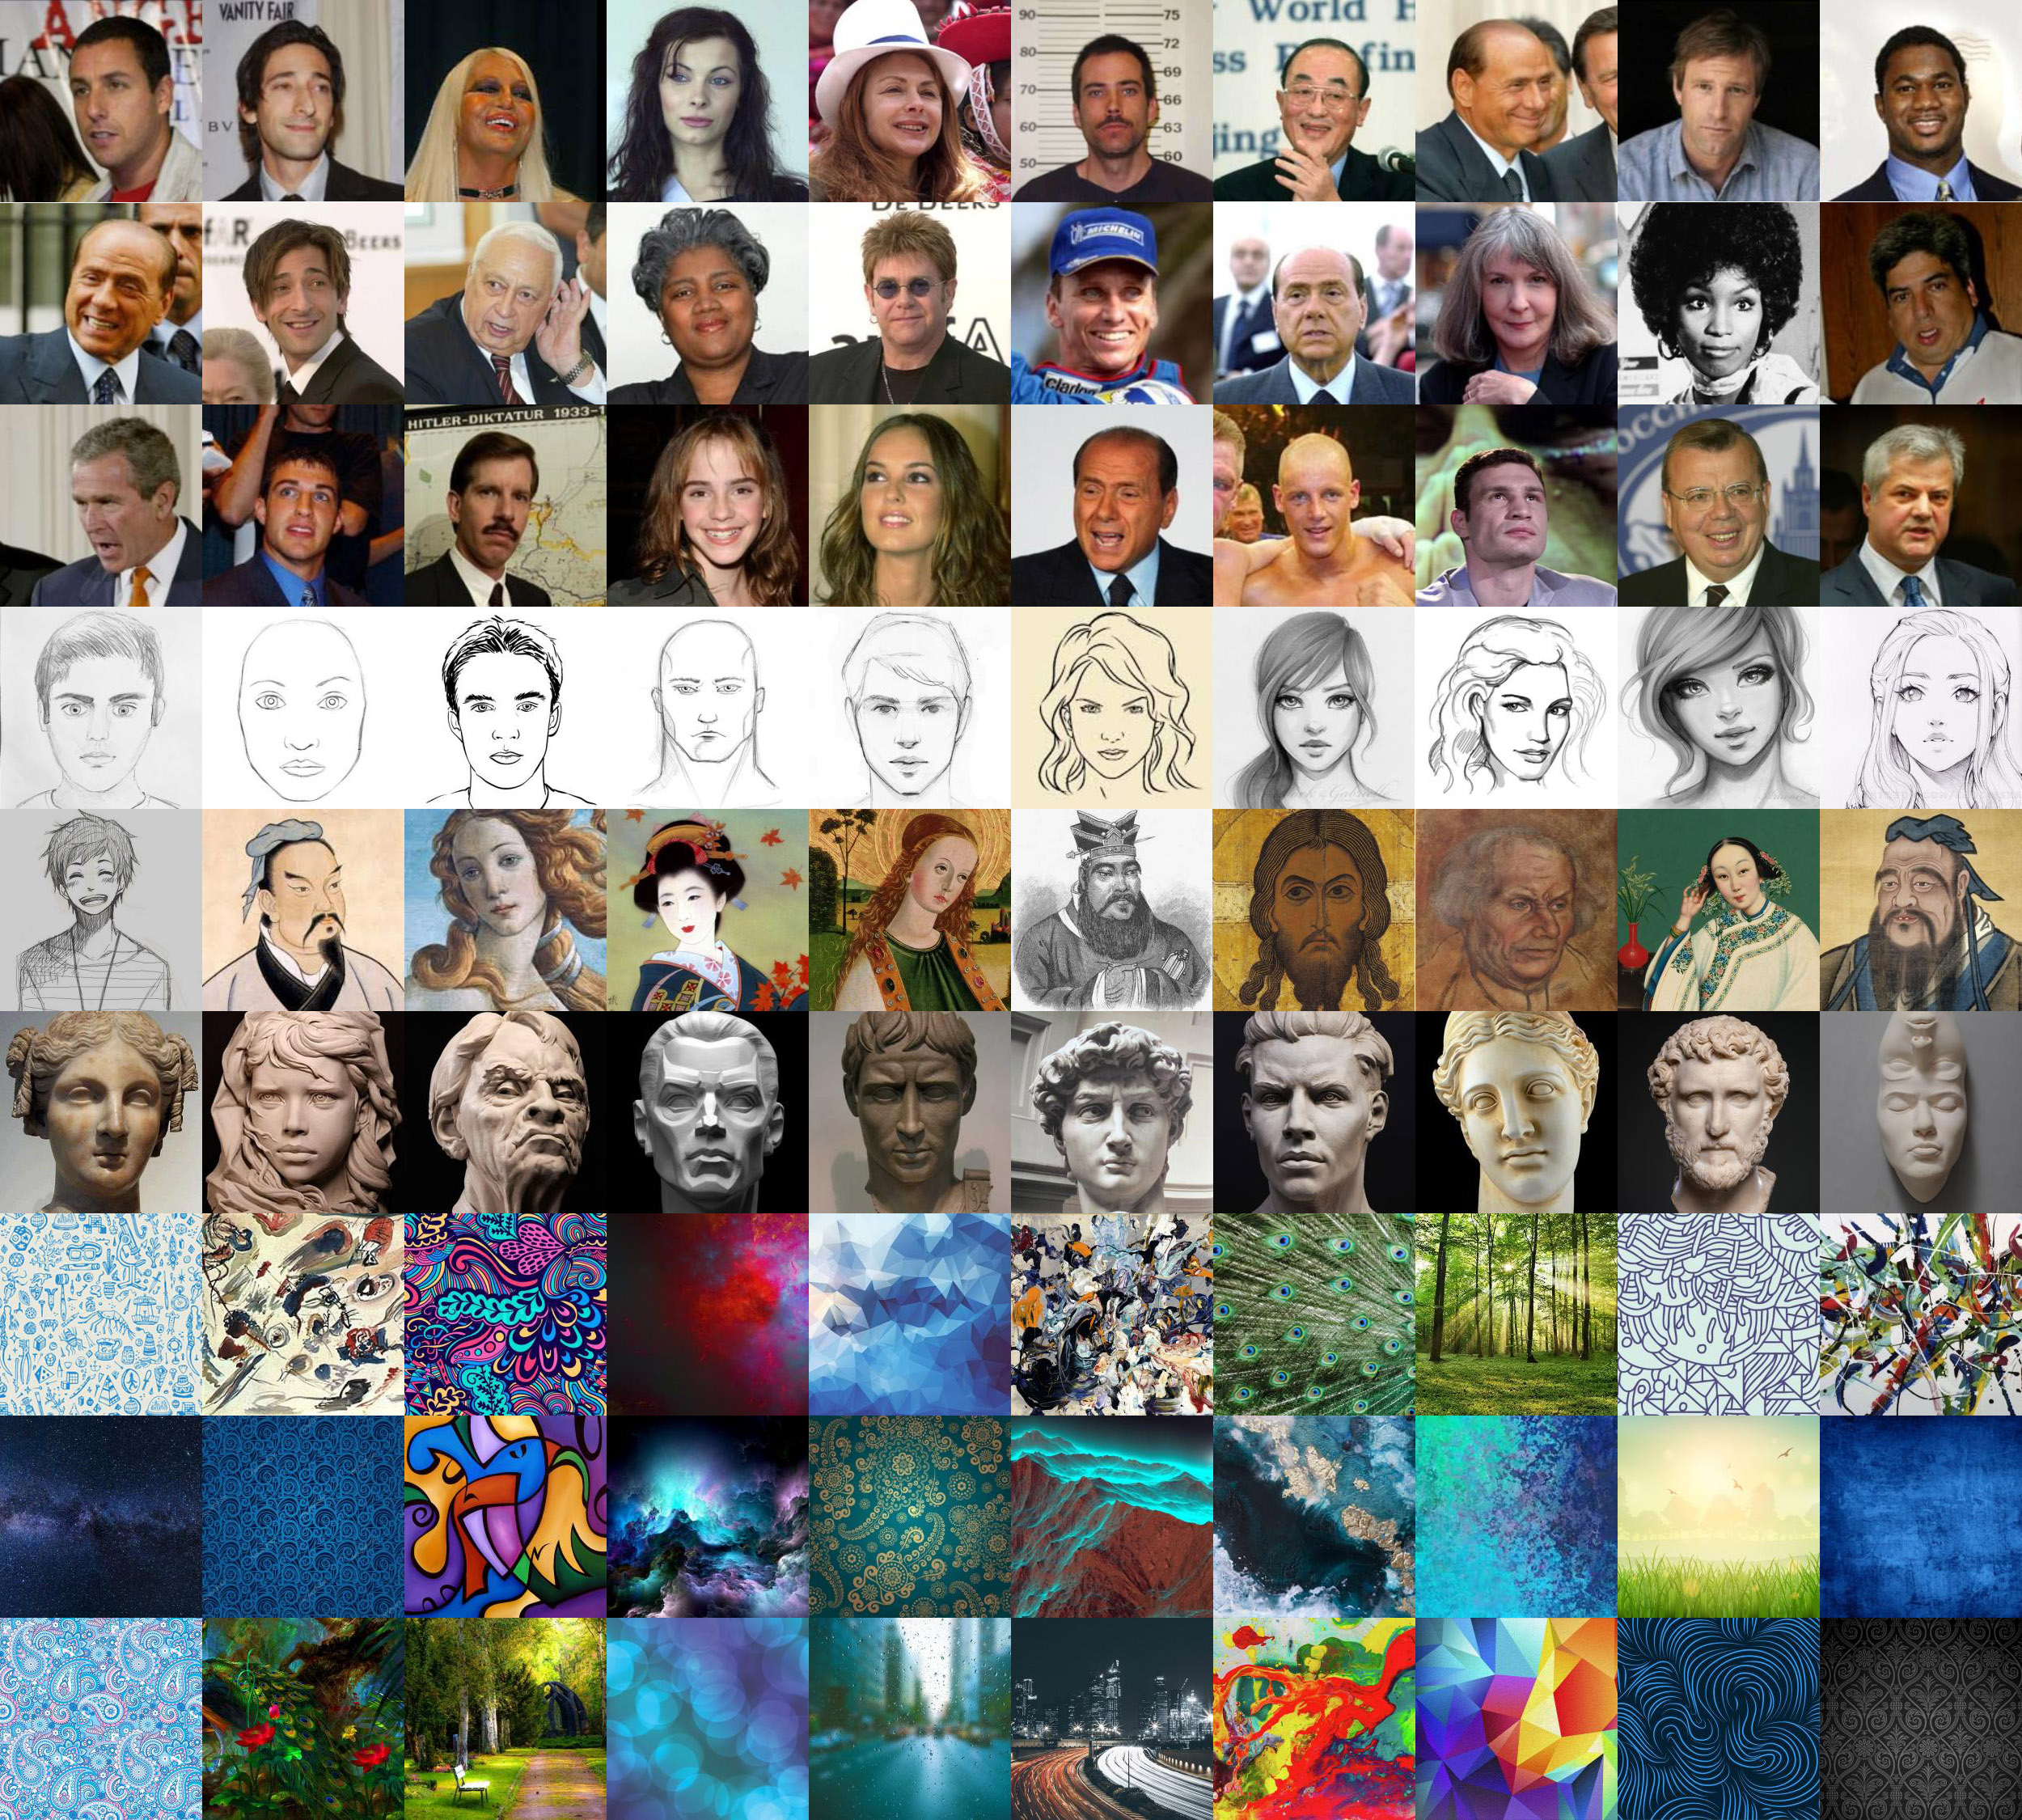
\includegraphics[width=14cm]{emp_studies/fd_dataset}
	%	\caption{Dataset for the Experiment 1}
	%	\label{fig:fd_dataset}
	%\end{figure}

	\subsection{Results}
	The results of the experiment are shown in the Table \ref{table:experiment_1_res}, where the rows refer to the prediction of the classifier and the columns refer to the three different datasets (in the case of the near-face dataset, each sub-group is shown in a different column).

	\begin{table}[H]
		\centering
		\resizebox{\textwidth}{!}
		{		
		    \begin{tabular}{L{3.5cm} | R{2.7cm} | R{0.9cm} | R{0.9cm} | R{0.9cm} | R{2.7cm} |}
			    \cline{2-6}
			    & \multicolumn{1}{c|}{Face dataset} & \multicolumn{3}{c|}{Near-face dataset} & \multicolumn{1}{c|}{Non-face dataset} \\ 
			    \hline
			    \multicolumn{1}{|c|}{Face detected} 	& 27 		& 6 & 6 & 10 		&  0 \\
				\hline
				\multicolumn{1}{|c|}{Face not detected} &  3 		& 5 & 3 &  0 		& 30 \\
				\hline
			\end{tabular}
		}
		\caption{Results of the Experiment 1}
	    \label{table:experiment_1_res}
	\end{table}

	% Look up confusion matrix, precision and recall
	\subsection{Evaluation}

\section{Effectiveness of Convolutional Neural Networks for Face Recognition}
	\subsection{Objective}
	%How many faces are correctly recognised?
	%How many faces are missed (false negatives)?
	\subsection{Method and parameters}
	%50 images of Mario: different illumination, pose, rotation, scale.
	\subsection{Data set}
	\subsection{Results}
	% Look up confusion matrix, precision and recall
	\subsection{Evaluation}



